\chapter{Presentation, Analysis and Interpretation of Data}
\chaptermark{Presentation, Analysis and Interpretation}
	This chapter details the functionalities of the developed system, including its user interface design. Moreover, the system answers the optimal shelter location-allocation for Calumpit. It also presents the evaluation results gathered from the LGU and IT experts, assessing the system’s acceptability and alignment with local needs.

\section{The Developed System}
	The researchers and developers of this thesis developed a decision support system to optimize shelter location allocation since there was a lack of system development. Identifying the most optimal shelter facility for a community is the system's main function. Specifically, it has five key features that let users completely modify the input parameters, and output processing. 


\subsection{Data Modification}
	The process of creating, updating, or deleting data within the system to maintain accuracy and relevance. This ensures that all records are up-to-date and properly managed so they can effectively be used for shelter allocation.
	
	\begin{figure}[h!]
		\caption{Dashboard}
		\centering
		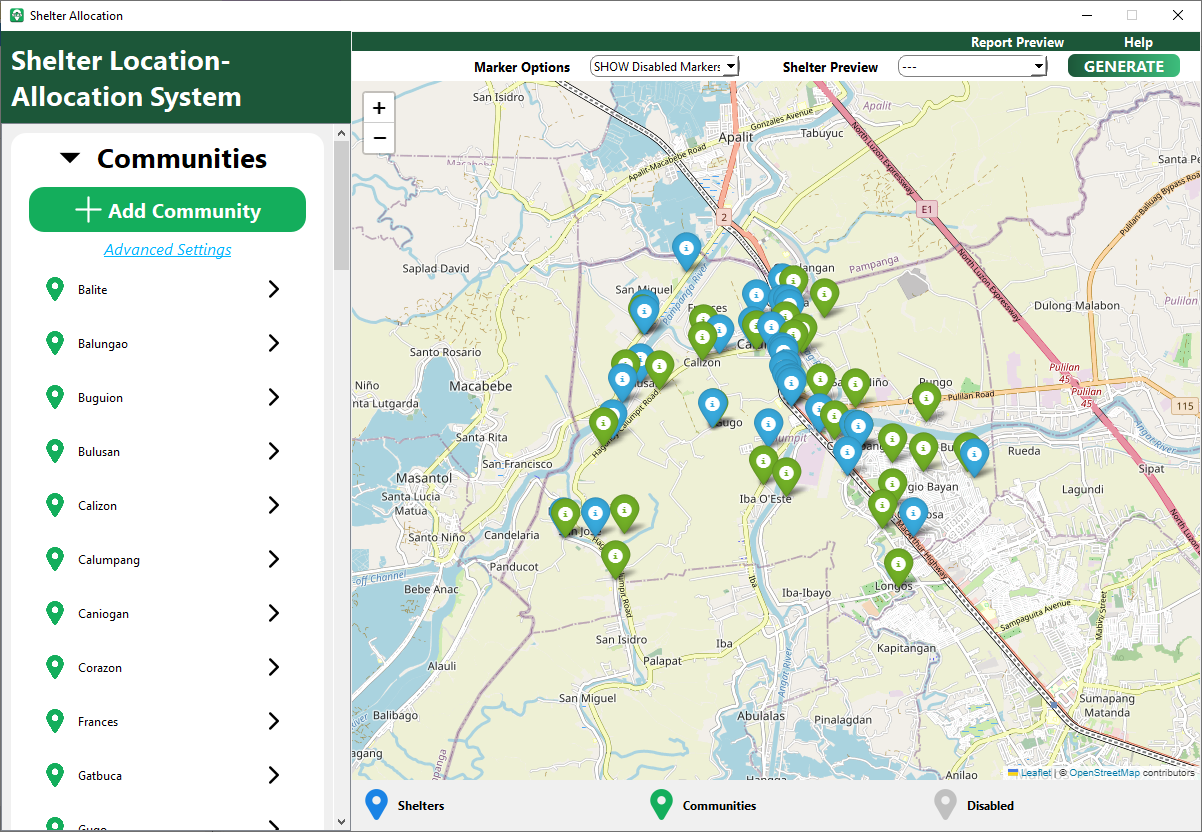
\includegraphics[width=3.5in]{Chapter 4/dashboard}
		\label{db}
	\end{figure}
	The dashboard provides an overview of a list of shelters and communities as shown in figure \ref{db}. It also displays a map where shelters and communities are pinned. Users can see whether a shelter is active or inactive. Additionally, the user can manipulate the map to filter and display only active shelter as well as shelters that are built, partially built, damaged, empty lot, and resistance to flood, typhoon, and earthquake
	
	\begin{figure}[h!]
		\caption{Community Management}
		\centering
		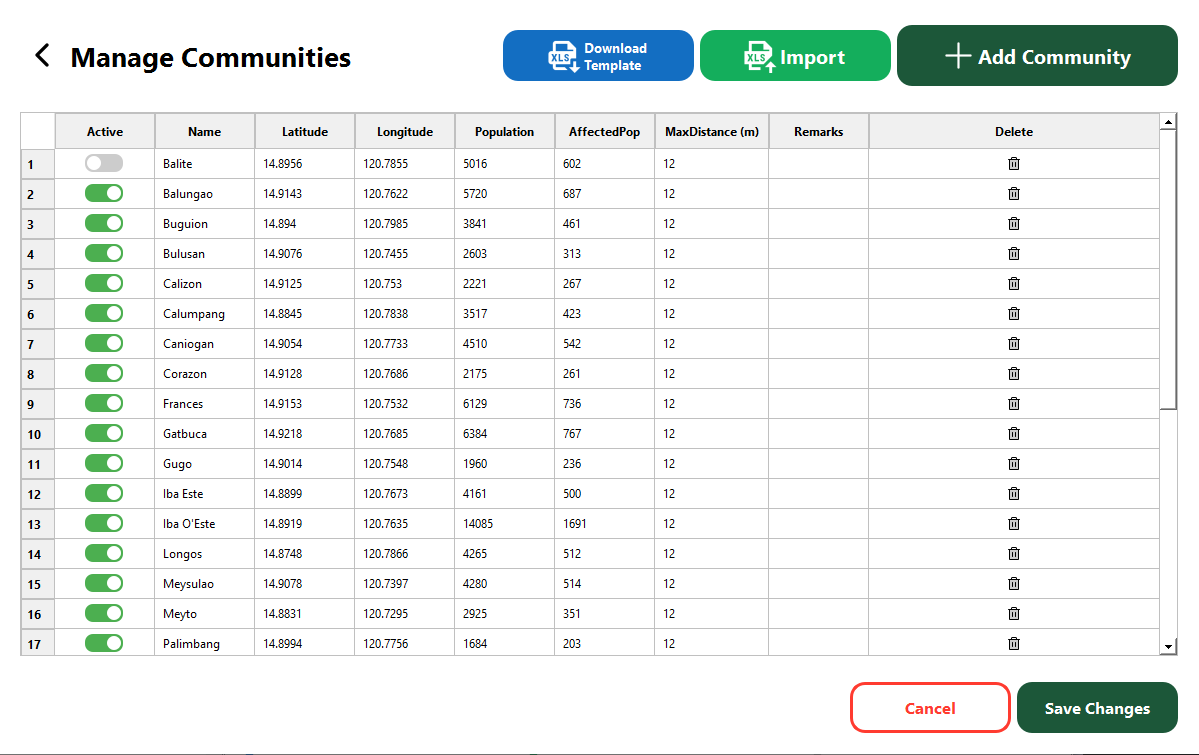
\includegraphics[width=3.5in]{Chapter 4/commadvanced}
		\label{commMan}
	\end{figure}
	Community management module manages the recorded details of barangays as shown in figure \ref{commMan}. It displays whether a barangay is active or inactive, along with its latitude, longitude, population, affected population, maximum distance, remarks, and a delete button. Users can also add new communities, download a template to ensure correct formatting when importing data, and manage barangay-related information efficiently.
	
	\begin{figure}[h!]
		\caption{Shelter Management}
		\centering
		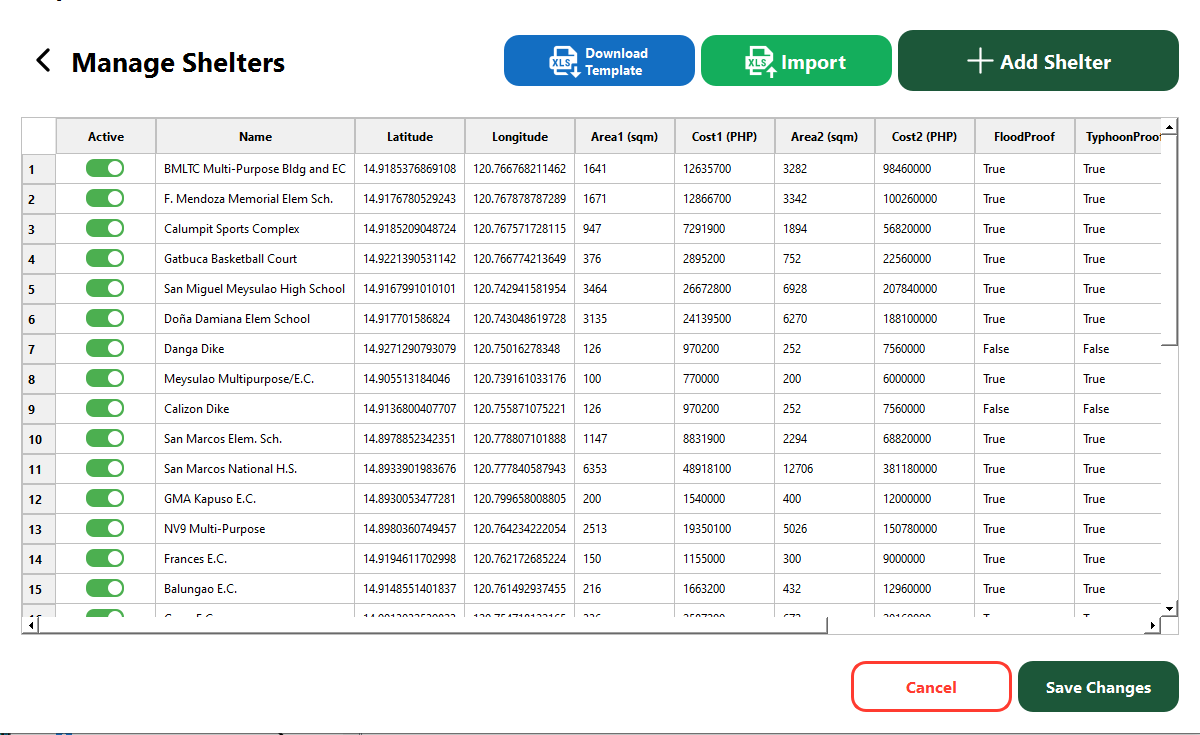
\includegraphics[width=3.5in]{Chapter 4/sheladvanced}
		\label{shelMan}
	\end{figure}
	The shelter management module, as shown in figure \ref{shelMan}, is similar to community management but includes different data fields. It contains information such as the shelter’s name, latitude, longitude, and classification as a Level 1 or Level 2 shelter. The module also tracks the cost of construction and maintenance for each level. Additionally, it indicates whether the shelter is resistant to floods, typhoons, and earthquakes. Users can also view the shelter’s status – whether it is built, partially built, damaged, or an empty lot.
	
\subsection{Model Modification}
	This concerns the parameters to be used in the model that may be modified for a more ideal setup depending on the preferences of the user. The parameters that may be changed here include the area per individual based on meters squared, the max number of level 2 shelters and shelters in general, the weights for both distance and cost, the number of generations, the number of populations in a generation, and the mutation rate. Measures are put in place to prevent entering of wrong values in these parameters such as letters or negative numbers. 
	
	\begin{figure}[h!]
		\caption{Model Parameter Settings}
		\centering
		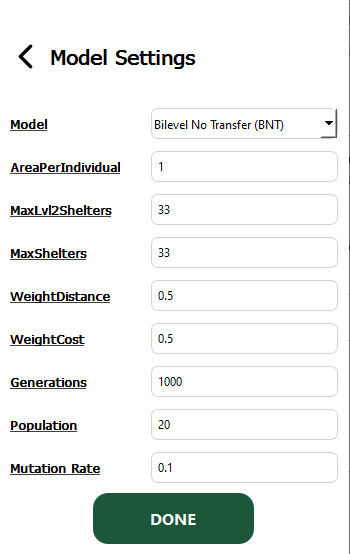
\includegraphics[width=3.5in]{Chapter 4/modelsettings}
		\label{modelSet}
	\end{figure}
	These factors impact the time taken to simulate data as well as the efficiency of the simulation, it is recommended to keep the parameters at default values unless the user is knowledgeable about the model or the system. These parameters are modified in the Model Settings module as shown in figure \ref{modelSet}, which may be accessed from the Solve Settings module by clicking Advanced Settings below Model.
	
	
\subsection{Data Simulation}
	This pertains to solving the model by running the Genetic Algorithm, which determines the most optimal shelter location allocation. As the core functionality of the system, it processes input data of communities and shelters, applies defined model parameters, then generates and displays the best allocation of the municipality.
	
	\begin{figure}[h!]
		\caption{Progress Dialog}
		\centering
		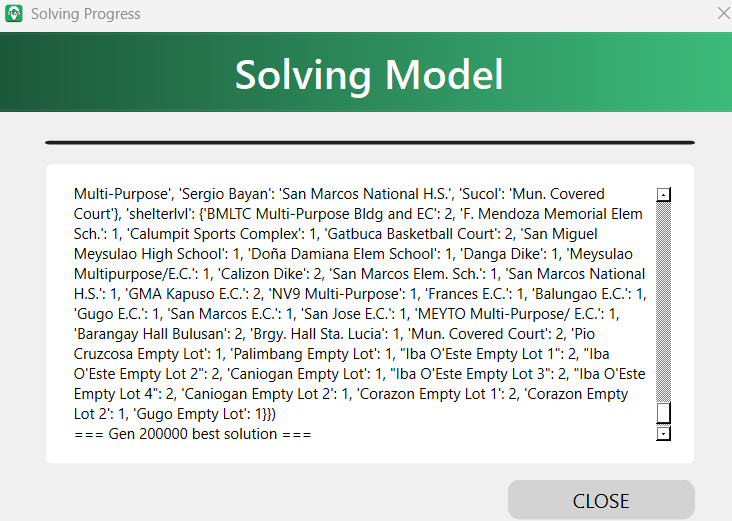
\includegraphics[width=3.5in]{Chapter 4/progress}
		\label{solveProg}
	\end{figure}
	Progress dialog as shown in figure \ref{solveProg} provides real-time logs and tracks the progress of the simulation. The process starts by computing the distances between each community and each shelter using a Python library, OSMnx. Once the distances are calculated, the system proceeds with the Genetic Algorithm to optimize the allocation. Users also have the option to cancel the process at any time.
	
	\begin{figure}[h!]
		\caption{Report Dialog}
		\centering
		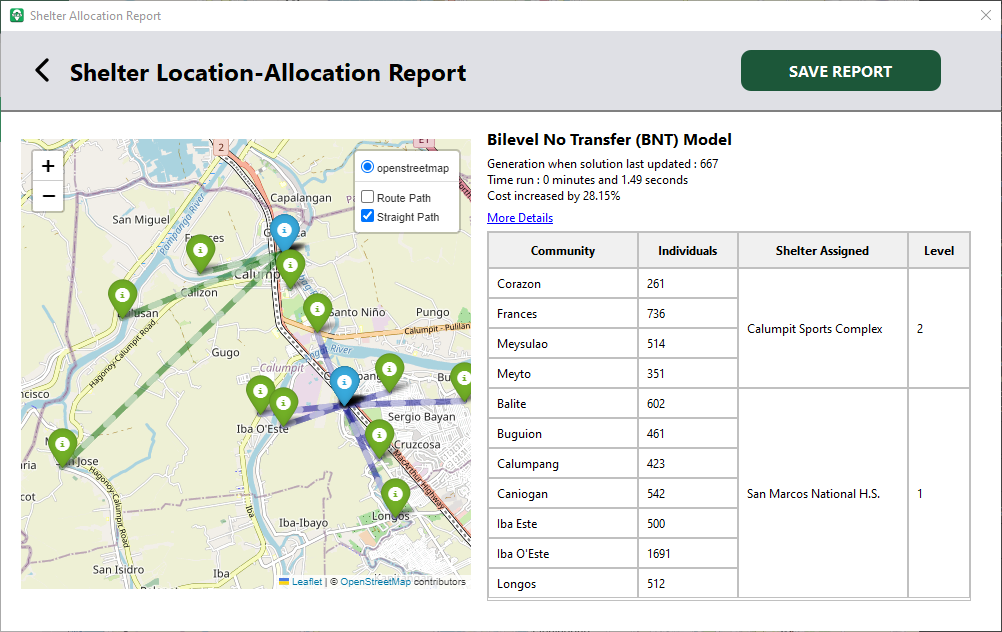
\includegraphics[width=3.5in]{Chapter 4/alloc report}
		\label{shelAllocRep}
	\end{figure}
	After the solving process is completed, report dialog appears displaying the final allocation results as shown in figure \ref{shelAllocRep}. It shows which communities are assigned to shelters, and displays the paths they can take on a map. This helps users analyze the feasibility and efficiency of the allocation.
	
	The Genetic Algorithm is implemented from scratch using Python, ensuring full control over its functionality and optimization process. The main functions in the code include fitness calculation, constraint enforcement, and the implementation of selection, mutation, and crossover.
	
	Appendix \_ details the fitness calculation, which represents the model's objective value. The first loop calculates the total distance, while the second loop determines the cost based on the level of the opened shelters.
	
	Appendices \_, \_, \_, and \_ implement the constraint functions, adding penalties to the objective value when violated. These constraints include maximum distance constraint, initial capacity constraint, maximum number of level 2 shelters that can be constructed/allocated, maximum number of shelters that can be constructed/allocated. Since the implemented Genetic Algorithm operates on integers, the constraints ensuring that each community is assigned only one shelter and one level are already satisfied.
	
\subsection{Shelter Tagging}
	This concerns the classification of shelters based on both structural resilience and current condition, ensuring shelters are appropriately assigned to communities based on availability, cost, and risk levels. Shelters are categorized in both resistance capabilities and status; resistance capabilities include flood-resistant, typhoon-resistant, and earthquake-resistant, and are not mutually exclusive to one another, for example, a shelter can be both flood and typhoon resistant. In terms of status, shelters can be built, partially built, damaged, and empty lots, each with varying costs depending on maintenance and construction.
	
	\begin{figure}[h!]
		\caption{Solve Settings}
		\centering
		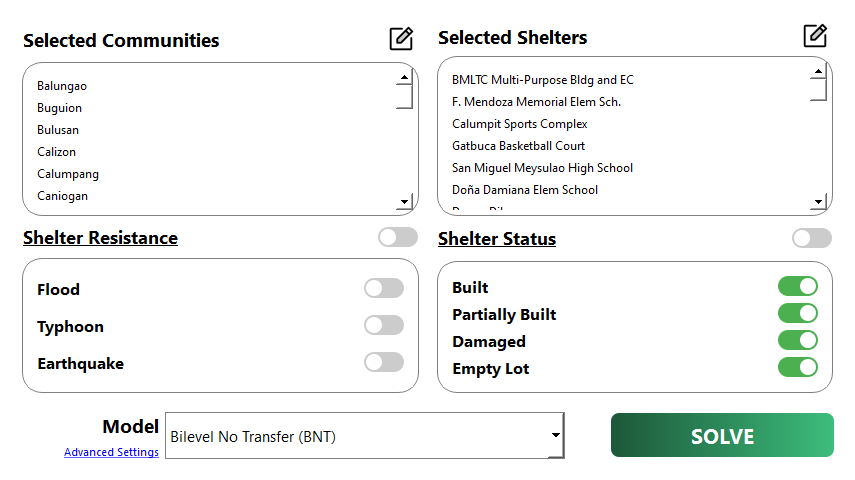
\includegraphics[width=3.5in]{Chapter 4/solvesettings}
		\label{solveSet}
	\end{figure}
	Selecting shelters with specific resistances and statuses in mind is done in the Solve Settings module as shown in figure \ref{solveSet}, where selecting or deselecting a specific resistance will remove shelters that do not meet the criteria from the data simulation. This ensures users will not assign communities to shelters that are not suited to the situation. Users may also check the status and resistances of a specific shelter in either the dashboard module by selecting a shelter, or in the shelter advanced settings, displaying all shelters’ statuses.
	

\subsection{Report Protection}
	To maintain confidentiality and prevent the unauthorized modification of reports, a security mechanism has been implemented in the system. This module includes password authentication, report encryption and identification of the creator of a report based on device-specific attributes.
	
	\begin{figure}[h!]
		\caption{Input Password Popup}
		\centering
		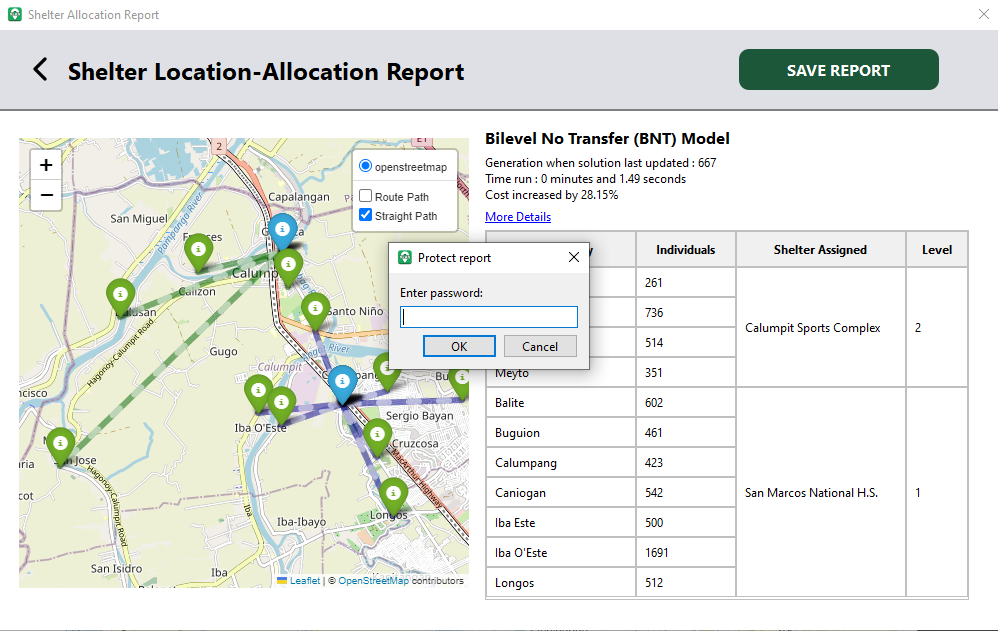
\includegraphics[width=3.5in]{Chapter 4/alloc report pass}
		\label{passPop}
	\end{figure}
	Upon finishing data simulation, the generated report may be saved in an excel format, and gives users the option to add password protection to the file through a popup as shown in figure \ref{passPop}. This ensures only intended users may access the report, the generated excel file itself is also read-only, without the ability to modify the data without authorization. The protected file was encrypted using a Python library, MSoffcrypto.
	
	The excel file also contains identification of the creator of the report, containing three device-specific identifiers, the IP address or the location of the user’s device, the MAC address or the identifier of the user’s network interface, as well as the name of the device the report was generated in. This information is logged in the password protected excel file, enhancing security and ensuring unauthorized users are logged and tracked. 
	
\section{Generated Shelter Location-Allocation Report}
	This section discusses the process of generating reports for shelter location allocation. The report helps in optimizing shelter assignments for communities based on various parameters and ensuring efficient disaster response. The data used considers only 12\% of the population in each barangay as affected. Additionally, the shelters have a maintenance cost, which are factored into the optimization process.
	
	The higher the number of generations, the more accurate the results in allocating communities to shelters. Running 200,000 generations improves optimization, ensuring better placement of communities in suitable shelters.
	
	\begin{table}[h]
		\centering
		\caption{Model Parameters}
		\label{modelParams}
		\begin{tabular}{|c|c|}
			\hline
			\textbf{Parameter} & \textbf{Value} \\ \hline
			Area Per Individual & 1 \\ 
			Maximum Level 2 Shelters  & 33 \\ 
			Maximum Shelters & 33 \\ 
			Weight Distance & 0.5 \\ 
			Weight Cost & 0.5 \\ 
			Generations & 200000 \\ 
			Population & 100 \\ 
			Mutation Rate & 0.1 \\ \hline
		\end{tabular}
	\end{table}
	
	\begin{table}[h]
		\centering
		\caption{Generated Shelter Location-Allocation for Calumpit}
		\label{calReport}
		\begin{tabular}{|c|c|c|}
			\hline
			\textbf{Community} & \textbf{Shelter Assigned} & \textbf{Level} \\ \hline
			Calizon & \multirow{5}{*}{Dona Damiana Elem School} & \multirow{5}{*}{Level 1} \\ \cline {1-1} 
			Frances & & \\ \cline {1-1} 
			Gatbuca & & \\ \cline {1-1} 
			Meysulao & & \\ \cline {1-1} 
			San Miguel  & & \\ \hline
			
			Bulusan & \multirow{6}{*}{Mun. Covered Court} & \multirow{6}{*}{Level 2} \\ \cline {1-1} 
			Corazon & & \\ \cline {1-1} 
			Panducot & & \\ \cline {1-1} 
			Poblacion & & \\ \cline {1-1} 
			Santa Lucia & & \\ \cline {1-1} 
			Sucol & & \\ \hline
			
			Balungao & \multirow{5}{*}{NV9 Multi-Purpose} & \multirow{5}{*}{Level 1} \\ \cline {1-1} 
			Meyto & & \\ \cline {1-1} 
			San Jose & & \\ \cline {1-1} 
			Santo Niño & & \\ \cline {1-1} 
			Sapang Bayan & & \\ \hline
			
			Caniogan & \multirow{3}{*}{San Marcos Elem. Sch.} & \multirow{3}{*}{Level 1} \\ \cline {1-1} 
			Palimbang & & \\ \cline {1-1} 
			San Marcos & & \\ \hline
			
			Balite & \multirow{10}{*}{San Marcos National H.S.} & \multirow{10}{*}{Level 1} \\ \cline {1-1} 
			Baguion & & \\ \cline {1-1} 
			Calumpang & & \\ \cline {1-1} 
			Gugo & & \\ \cline {1-1} 
			Iba Este & & \\ \cline {1-1} 
			Iba O'Este & & \\ \cline {1-1} 
			Longos & & \\ \cline {1-1} 
			Pio Cruzcosa & & \\ \cline {1-1} 
			Pungo & & \\ \cline {1-1} 
			Sergio Bayan & & \\ \hline
		\end{tabular}
		
	\end{table}
	
	\begin{figure}[h!]
		\caption{Community to Shelter Straight Path}
		\centering
		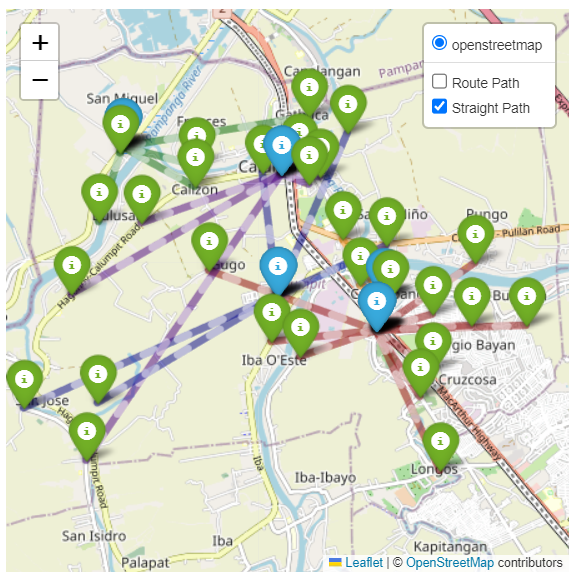
\includegraphics[width=3.5in]{Chapter 4/straight path}
		\label{straightpath}
	\end{figure}
	
	\begin{figure}[h!]
		\caption{Community to Shelter Route Path}
		\centering
		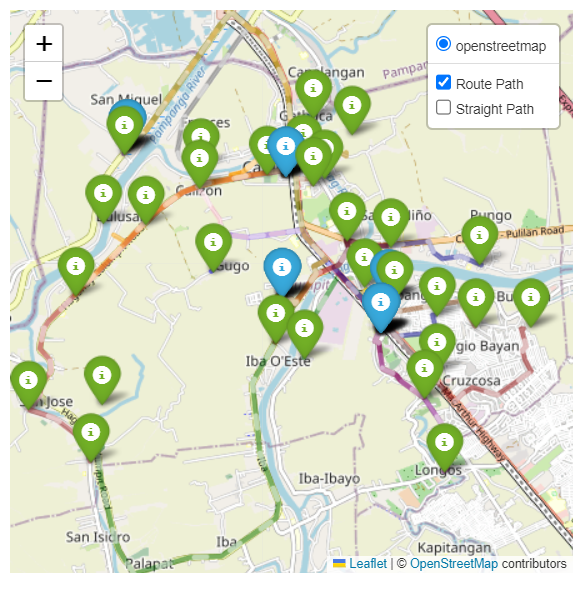
\includegraphics[width=3.5in]{Chapter 4/route path}
		\label{routepath}
	\end{figure}
	
	The generated report can be downloaded as an Excel file. In the Report Module, a map displays where communities are allocated to their designated shelters. Table \ref{calReport} provides detailed information, including communities, number of affected individuals which is 12\% of the population, assigned shelters, and shelter level. Figure \ref{straightpath} and \ref{routepath} shows the generated map which visualizes the allocation result.
	
	

%\section{System Evaluation}
%
%Present a summary of the evaluation of your system by the IT Experts and the End-users, then discuss the analysis and interpretation of the result. Summarize the feedback received from users and describe any improvements made to the system based on user feedback. You may divide the discussions in subsections for a clearer structure.
%
%\begin{table}[ht]
%	\centering
%	\caption{Example of a Table in APA Format}
%	\label{tab:apaformat}
%	\begin{tabularx}{\linewidth}{X*{4}{>{\centering\arraybackslash}X}}
%		\toprule
%		\multirow{2}{*}{\textbf{Column 1}} & \multicolumn{2}{c}{\textbf{Merge Column 2 \& 3}} & \multicolumn{2}{c}{\textbf{Merge Column 4 \& 5}}\\
%		\cmidrule(lr){2-3} \cmidrule(lr){4-5}
%		& Decription 1 & Description 2 & Variant 1 & Variant 2\\
%		\midrule
%		Variable 1 & xxx.xx & xx.xx & xxxx.xx & x.xx\\
%		Variable 2 &  xx.xx & xxxx.xx& x.xx & xxx.xx\\
%		Variable 3 & xxxx.xx & x.xx & xxx.xx & xx.xx\\
%		Variable 4 &  x.x & xxx.xx & xx.xx & xxxx.xx\\
%		\midrule
%		TOTAL & \textbf{xxxxx.xx} & \textbf{xxxx.xx} & \textbf{xxxx.xx} & \textbf{xxxx.xx}\\
%		\bottomrule
%	\end{tabularx}
%\end{table}